%%%%%%%%%%%%%%%%%%%%%%%%%%%%%%%%%%%%%%%
\chapter{Spielformen und Trainingsspiele}
\label{spielformen}

Todo: Ergänzen http://lukck.blogspot.de/2015/06/inhaltsverzeichnis.html

Im Tischfußball gibt es Wettkämpfe für drei Disziplinen: 
\begin{itemize}
\item \nameref{spielformen:npersonen:einzel}
\item \nameref{spielformen:npersonen:doppel}
\item \nameref{spielformen:npersonen:team}
\end{itemize}
Neben diesen Grundspielformen gibt Varianten, die zum Training da sind und Spaß machen. Dabei wird in drei Bereichen unterteilt:
\begin{itemize}
\item \nameref{spielformen:zaehlweisen}
\item \nameref{spielformen:npersonen}
\item \nameref{spielformen:sonderregeln}
\end{itemize}
Die jeweiligen Spielformen werden in diesem Kapitel vorgestellt. Darüberhinaus kann man sich neue Varianten ausdenken, in dem man Spielformen der drei Bereiche kombiniert: Man legt fest, wie man zählt, mit wie vielen Personen man spielt und mit welchen etwaigen Sonderregeln.

\paragraph{Didaktischer Hintergrund:} Diese Variationen bieten sich insbesondere für das sogenannte {\normalfont \itshape  genetische Lernen} in Gruppen an: Nach dem Spielen einer Spielform wird gemeinsam reflektiert, was gut war und wo der Spaß eventuell zu kurz kam. Gemeinsam wird diskutiert, welche Sonderregeln und Spielformen beim naechsten Mal festgelegt werden, um den Spaß in der Gruppe hoch zu halten und das spielerische Lernen attraktiv zu machen. 

%%%%%%%%%%%%%%%%%%%%%%%%%%%%%%%%%%%%%%%
%%%%%%%%%%%%%%%%%%%%%%%%%%%%%%%%%%%%%%%
\section{Zählweisen}
\label{spielformen:zaehlweisen}

Beim Tischfußball muss man Tore schießen und am besten mehr als sein Gegenspieler, um am Ende zu gewinnen.
Es gibt jedoch verschiedene Zählweisen, auf die man sich vor Beginn des Spiels einigt oder die bei Turnieren gespielt werden. 

%%%%%%%%%%%%%%%%%%%%%%%%%%%%%%%%%%%%%%%
\subsection{Ein Satz}
\label{spielformen:zaehlweisen:einsatz}

Wenn man einfach so kickert ohne ein Turnier zu spielen, spielt man oft einen Satz bis 6 Tore: Wer zuerst 6 Tore geschossen hat, gewinnt die Partie.
Als wichtigste Variante gilt die Unentschiedenregel: Bei 5 zu 5 Toren geht der Satz unentschieden aus.

\paragraph{Hintergrund:}
Obwohl bei vielen Tischmodellen die Torzähler 10 Tore zählen können, wird meistens bis 6 Tore gespielt -- aber auch ein Satz bis 5 oder 7 Toren sind verbreitet.
Spiele, die über einen Satz gehen, werden bei Turnieren oft in der Vorrunde gespielt.


%%%%%%%%%%%%%%%%%%%%%%%%%%%%%%%%%%%%%%%
\subsection{Mehrere Gewinnsätze}
\label{spielformen:zaehlweisen:gewinnsaetze}

Wie beim Tennis, spielt man bei Tischfußballpartien über mehrere Gewinnsätze -- das heißt, wer zuerst eine festgelegte Anzahl von Sätzen gewinnt, gewinnt die Partie. Am gängigsten sind:
\begin{itemize}
\item Zwei Gewinnsätze (engl. "Best of three"): Derjenige, der zuerst zwei Sätze gewinnt, gewinnt die Partie. Mit 2:0 Sätzen hat man also gewonnen. 
Es können maximal drei Sätze gespielt werden: Falls es nach den ersten beiden Sätzen 1:1 steht, gibt es einen dritten entscheidenden Satz, und die Partie geht 1:2 oder 2:1 aus. 
\item Drei Gewinnsätze (engl. "Best of five"): Derjenige, der zuerst drei Sätze gewinnt, gewinnt die Partie, beispielsweise 3:1. Steht es 2:2 nach den ersten vier Sätzen, gibt es einen fünften und entscheidenden Satz. 
\end{itemize}
Die Sätze werden hier jeweils bis 5 Tore gespielt. Kommt es zu einem Entscheidungsatz, also in Satz 3 bei zwei Gewinnsätzen oder in Satz 5 bei drei Gewinnsätzen, gibt es eine Verlängerung, wenn es 4:4 Tore steht: Jetzt braucht man zwei Tore Vorsprung, um den letzten Satz und damit die Partie zu gewinnen. Bei drei Gewinnsätzen kann eine sehr knappe Partie zum Beispiel 4:5, 5:4, 4:5, 5:4 und 8:6 in Toren und damit 3:2 in Sätzen ausgeht. 

\paragraph{Hintergrund:}
Mehrere Gewinnsätze werden oft bei Turnieren in der KO-Runde gespielt. Hierbei setzt sich am Ende meist das bessere Team durch. 
Und: Bei manchen Tischmodellen sind extra Satzzähler neben den Torzählern angebracht. 




%%%%%%%%%%%%%%%%%%%%%%%%%%%%%%%%%%%%%%%
%%%%%%%%%%%%%%%%%%%%%%%%%%%%%%%%%%%%%%%
\section{Anzahl der Spieler}
\label{spielformen:npersonen}

Tischfußball kann man mit unterschiedlich vielen Spielern spielen. 
Neben den drei Grundspielformen 
\begin{itemize}
\item \nameref{spielformen:npersonen:einzel},
\item \nameref{spielformen:npersonen:doppel} und 
\item \nameref{spielformen:npersonen:team}, 
\end{itemize}
gibt es auch die Möglichkeit mit drei, fünf, sechs, sieben, acht oder sogar mehr Personen an einem Tisch zu kickern.
Hierbei wird ansonsten nach den normalen \nameref{regeln} gespielt.

Hat man einen Spielmodus gewählt, kann man damit ein Training oder \nameref{turniere} gestalten, sodass möglichst alle Teilnehmer viele Spiele machen können. 


%%%%%%%%%%%%%%%%%%%%%%%%%%%%%%%%%%%%%%%
\subsection{Einzel}
\label{spielformen:npersonen:einzel}

\begin{itemize}
\item Spieleranzahl: 2
\item Aufstellung: Eins gegen eins; jeder bedient mit seinen zwei Händen seine vier Stangen.
%\item Regeln: Normale \nameref{regeln} 
\item {\normalfont \bfseries Hintergrund:} Nur in der Einzel-Disziplin, der Doppel-Disziplin und der Team-Disziplin werden Titel vergeben: Landesmeister, Deutscher Meister und Weltmeister!  
\end{itemize}
 
%%%%%%%%%%%%%%%%%%%%%%%%%%%%%%%%%%%%%%%
\subsection{Doppel}
\label{spielformen:npersonen:doppel}

\begin{itemize}
\item Spieleranzahl: 4
\item Aufstellung: Zwei gegen zwei; jedes Team hat einen Torwart, der die 1er- und 2er-Stange bedient, und einem Stürmer, der die 5er- und 3er-Stange bedient.
%\item Regeln: Normale  \nameref{regeln} 
\item {\normalfont \bfseries Hintergrund:} Es ist nicht klar, welches die Königsdisziplin im Tischfußball ist: Einzel oder Doppel? Fest steht das gute Einzelspieler auch gute Doppelspieler sind und anders herum -- und auch gute Teamspieler: 
Bei den Weltmeisterschaften werden die Einzelweltmeister am Freitag, die Doppelweltmeister am Samstag und am Sonntag als Letztes und als Höhepunkt die Teamweltmeister ausgespielt. 
\end{itemize}

%%%%%%%%%%%%%%%%%%%%%%%%%%%%%%%%%%%%%%%
\subsection{Team}
\label{spielformen:npersonen:team}

\begin{itemize}
\item Spieleranzahl: 2mal mindestens 3 Spieler
\item Spielplan: Es gibt einen Spielplan mit Einzel- und Doppelpartien, die typerweise auf einen Satz mit Unentschieden. Zum Beispiel:
\begin{itemize}
\item Teamgröße: Jedes Team hat jeweils drei Spieler
\item Spielmodus: Es werden 6 Spiele gespielt, nämlich drei Einzel und drei Doppel im Wechsel: Einzel 1, Doppel 1, Einzel 2, Doppel 2, Einzel 3 und Doppel 3.
\item Aufstellung: Jeder spielt ein Einzel und zwei Doppel mit dem jeweils anderen, also in Doppel 1 spielen Einzel 2 und Einzel 3 Spieler zusammen, in Doppel 2 spielen Einzel 3 und Einzel 1 Spieler und in Doppel 3 spielen Einzel 1 und Einzel 2 zusammen.  
\item Ergebnis: Gewinnt man ein Spiel bekommt man 2:0 Punkte, bei Unentschieden gibt es 1:1 Punkte, und bei einer Niederlage 0:2 Punkte. Damit sind bei 6 Spielen insgesamt 12 Punkte zu vergeben. Eine Partie kann also z.B. 12:0 oder 7:5 oder 6:6 ausgehen. 
\end{itemize}
%\item Regeln: Normale Regeln 
\item Varianten: Je nach Teamgröße kann man den Spielplan und die Aufstellungsregeln variieren. 
\item {\normalfont \bfseries Hintergrund:} Bei der Team-Weltmeisterschaft werden zum Beispiel 4 Doppel und 2 Einzel gespielt und jeder Spieler darf maximal 1 Einzel und 1 Doppel spielen. Darum muss das Team aus mindestens 8 Spielern bestehen. 
\end{itemize}

%%%%%%%%%%%%%%%%%%%%%%%%%%%%%%%%%%%%%%%
\subsection{Kleine Runde (6 Personen)}
\label{spielformen:npersonen:kleine}

\begin{itemize}
\item Spieleranzahl: 6
\item Aufstellung: Jedes Team hat jeweils drei Spieler. Jeweils eine Doppelkombination spielt einen Ball, nach einem Tor rotiert jedes Team: Der Pausierende wird Torwart, der Torwart wird Stürmer und der Stürmer pausiert den nächsten Ball, usw.
\item Trainingseffekt: Konzentration auf ein Ball und eine Position, Zusammenspiel, Spaß, Teambuilding
\item Variation: Zu fünft kann man alternativ ein festes Doppel (2 Spieler) gegen eine rotierendes 3er-Team spielen.
\end{itemize}

%%%%%%%%%%%%%%%%%%%%%%%%%%%%%%%%%%%%%%%
\subsection{Vier gegen vier}
\label{spielformen:npersonen:viergegenvier}

\begin{itemize}
\item Spieleranzahl: 8
\item Aufstellung: Jeder greift mit einer Hand eine Stange.
Wenn ein Team ein Tor erzielt, wechselt dieses die Positionen: Jeder rückt
eine Stange vor und der Stürmer geht an die Torwartstange.
\item Trainingseffekt: Konzentration auf eine Hand, Zusammenspiel, Spaß
\item Variation: Alle nur die rechte Hand, oder nur die linke Hand
\end{itemize}

%%%%%%%%%%%%%%%%%%%%%%%%%%%%%%%%%%%%%%%
\subsection{Drei gegen drei (6 Personen)}
\label{spielformen:npersonen:dreigegendrei}

\begin{itemize}
\item Spieleranzahl: 6
\item Aufstellung: Jeder greift mit einer Hand eine Stange.
Innerhalb eines Teams darf die freie Stange durch Umgreifen aktiviert werden, allerdings
dürfen sich die Hände nicht überkreuzen.
Wenn ein Team ein Tor erzielt, wechselt dieses die Positionen: Jeder rückt
eine Stange vor und der Stürmer geht an die Torwartstange.
\item Trainingseffekt: Konzentration auf eine Hand mit mehreren Stangen, Zusammenspiel, Spaß
\item Variation: Alle nur die rechte Hand, oder nur die linke Hand. 
\end{itemize}

%%%%%%%%%%%%%%%%%%%%%%%%%%%%%%%%%%%%%%
\subsection{Zwei gegen eins}
\label{spielformen:npersonen:jedergegenjeden}

\begin{itemize}
\item Spieleranzahl:  3
\item Aufstellung: Ein Doppel (Torwart- und Stürmerposition) gegen ein Einzel, wobei die Spieler die Position während des Spiels wechseln.
Jeder sammelt für sich Punkte. Man erhält einen Punkt, wenn man in der
Einzelposition ein Tor schießt und dabei bleibt jeder bei seiner Position. 
Schießt das
aktuelle Doppelteam ein Tor, wird der Stürmer zum Einzelspieler, der Torwart zum
Stürmer, und der Einzelspieler zum Torwart („gegen den Uhrzeigersinn“).
\item Trainingseffekt: Einzeltraining, Passmöglichkeiten beim Doppel, schnelles Spiel
\end{itemize}


%%%%%%%%%%%%%%%%%%%%%%%%%%%%%%%%%%%%%%
\subsection{Runde (4 und mehr Personen)}
\label{spielformen:npersonen:runde}
\begin{itemize}
\item Spieleranzahl: 4 und am Besten mehr 
\item Aufstellung: Jeder hat eine Position, die restlichen Spieler verteilen sich auf beide Tischseiten und stellen sich hinter den Stürmer an: es wird gegen den Uhrzeigersinn gewechsel.
Gespielt wird normal bis ein Tor, danach verändern sich die Postionen:
\begin{itemize}
\item Beim Team, welches das Tor kassiert: Der Torwart fliegt raus, der Stürmer
wird Torwart, der nächste in der Schlange wird Stürmer.
\item Beim Team, welches das Tor schießt: Der Torschütze ist „gerettet“ und stellt
sich auf der anderen Seite hinten an. Schießt der Stürmer das Tor, wird der
nächste in der Reihe Stürmer und der Torwart bleibt. Schießt der Torwart
das Tor (oder fällt ein Eigentor oder ein nicht eindeutiges Tor), wird der
Stürmer Torwart, und der nächste in der Reihe Stürmer.
\item Es wird solange gespielt, bis nur noch zwei im Spiel sind. Diese spielen ein Einzel, bei dem derjenige eine Krone gewinnt, der zuerst 2 Tore schießt.
\end{itemize}
\item Trainingseffekt: Zusammenspiel, Spaß, Variation
\item Variation: jeder nur eine Stange, dann braucht man mehr als 8 Spieler
\end{itemize}


%%%%%%%%%%%%%%%%%%%%%%%%%%%%%%%%%%%%%%%
\subsection{Alleine am Tisch}
\label{spielformen:npersonen:alleine}

Wenn man mal alleine am Tisch steht, kann man sich auch selbst fordern, und eine Serie von 10 Versuchen spielen: Wie viele erfolgreiche Versuche schaffe?
Hier kann sich viele Serien ausdenken:
\begin{itemize}
\item Torschüsse: 
\begin{itemize}
\item Schieber, Zieher, Abroller oder Jet.
\item Von der 3er-Stange oder der 2er-Reihe.
\item Rechts- oder Linksschuss.
\item Kurze oder lange Schüsse.
\item Trickschüsse
\end{itemize}
\item Passen:
\begin{itemize}
\item Ins Feld, gerade oder an die Bande.
\item Kanten- oder Brushpass.
\item Von der 5er- auf die 3er-Stange.
\item Von der 2er-Stange auf die 3er-Stange.
\item Von der 2er-Stange auf die 5er-Stange.
\end{itemize}
\item Ballführung: 
\begin{itemize}
\item Ruhender Ball und Puppenwechsel.
\item Tictac oder Vorne-hinten Klemmen.
\item Auf der 2er-Stange zwischen der 1. und der 2. Puppe.
\item Auf der 3er-Stange zwischen der 1. und der 2. Puppe oder der 2. und der 3.Puppe oder mit der 1. und 3. Puppe.
\item Auf der 5er-Stange zwischen der zwei benachbarten Puppen oder mit zwei Puppen und dabei eine Puppe auslassen.
\end{itemize}
\end{itemize}
Hier kann man natürlich die Sicherheit, die Schnelligkeit und Schuss- und Passhärte mit Übung gezielt steigern.


%%%%%%%%%%%%%%%%%%%%%%%%%%%%%%%%%%%%%%%%
%%%%%%%%%%%%%%%%%%%%%%%%%%%%%%%%%%%%%%%%
%%%%%%%%%%%%%%%%%%%%%%%%%%%%%%%%%%%%%%%%
\section{Sonderregeln}
\label{spielformen:sonderregeln}

Hier findet ihr eine Sammlung an Spielarten, bei denen die normalen Regeln durch Sonderregeln ergänzt werden. 
Dadurch lernt man mit Spaß und spielerisch bestimmte Trainingsinhalte, da die Sonderregeln einen bestimmte Fokus setzen. 

%%%%%%%%%%%%%%%%%%%%%%%%%%%%%%%%%%%%%%%%
\subsection{Goalie-Einzel}
\label{spielformen:sonderregeln:goalie}

\begin{figure}
%\begin{wrapfigure}{r}{0.4\textwidth} 
\centering 
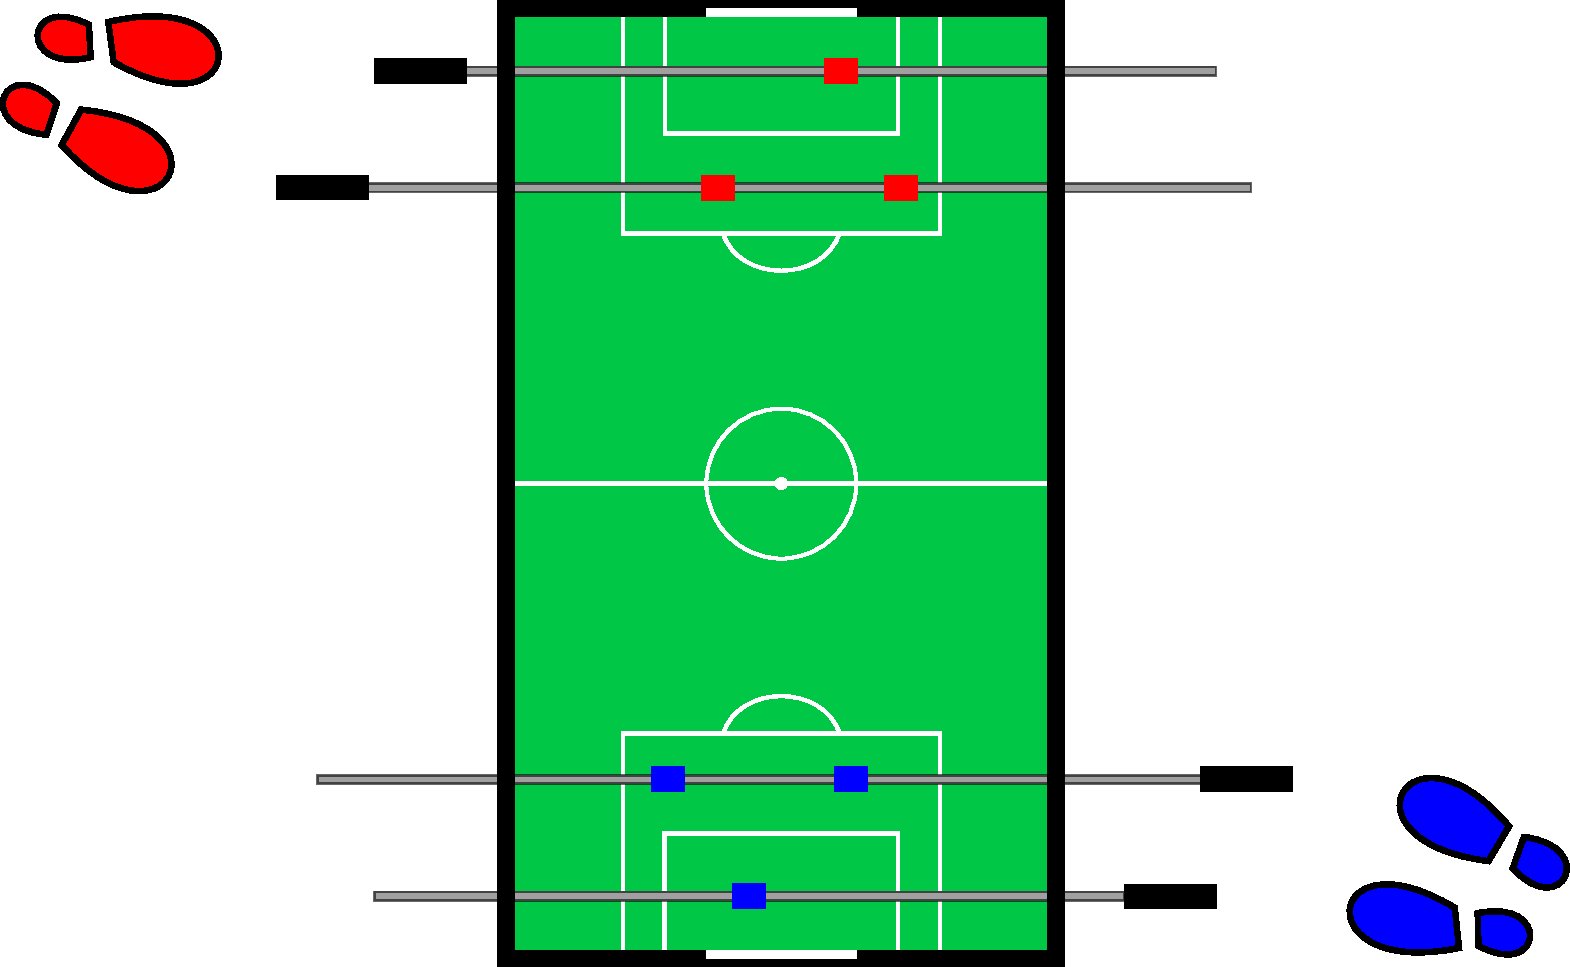
\includegraphics[width=0.38\textwidth]{img/spielform_goalie.pdf} 
\caption{Goalie-Einzel} 
\label{fig:goalie} 
\end{figure}
%\end{wrapfigure}

\begin{itemize}
\item Niveau: ab Anfänger
\item Spieleranzahl: 2
\item Aufstellung: 3er und 5er Stangen werden hochgeklappt und mit Rodlocks oder Haushaltsgummis fixiert (siehe auch \nameref{tisch:zubehoer:training}); ein Ball.
\item Regeln: Normale Regeln plus Sonderregel des Torwartbereichs: 
  \begin{itemize}
  \item Anstoß im Torwartbereich (siehe \nameref{spielformen:sonderregeln:abstoss}).
  \item Sobald der Ball den Torwartbereich verläßt und z.B. im mittleren Spielfeldbereich unerreichbar liegen bleibt, bekommt der Gegner den Ball und bringt den Ball neu ins Spiel.
  \item Springt der Ball aus dem Tisch, bekommt wie gewohnt derjenigen den Ball, der nicht rausgeschossen hat. 
  \end{itemize}
\item Trainingseffekt: defensive und offensive Grundlagen; Torwartdasein, wie Stellungsspiel, Ball stoppen und behalten; Ballführung und Spielfeldverständnis
%\item Variationen: \nameref{spielformen:sonderregeln:mehrerebaelle}, \nameref{spielformen:sonderregeln:unterschiedlichebaelle}, \nameref{spielformen:sonderregeln:onetouch}, \nameref{spielformen:sonderregeln:speedball}
\item Info: Goalie-Einzel wird bei vielen großen Turnieren als Nebendisziplin angeboten. Also selbst die Profis haben viel Spaß bei dieser Spielform.
\end{itemize}


%%%%%%%%%%%%%%%%%%%%%%%%%%%%%%%%%%%%%%%%
\subsection{Abstoß}
\label{spielformen:sonderregeln:abstoss}

\begin{itemize}
\item Niveau: ab Anfänger
\item Spieleranzahl und Aufstellung: variabel 
\item Regeln: Normale Regeln, aber der Anstoß nach einem Tor wird im Torwartbereich ausgeführt. 
\item Trainingseffekt: Vereinfachen des Spiels durch Weglassen des Anstosses auf der 5er-Reihe; mehr Spielanteile für den Torwart, wodurch das offensive Torwartspielen  gefördert wird
%\item Variationen: \nameref{spielformen:sonderregeln:dreigegendrei}, \nameref{spielformen:sonderregeln:unterschiedlichebaelle}, \nameref{spielformen:sonderregeln:onetouch}, \nameref{spielformen:sonderregeln:speedball}
\end{itemize}

%%%%%%%%%%%%%%%%%%%%%%%%%%%%%%%%%%%%%%%%
\subsection{Mehrere Bälle}
\label{spielformen:sonderregeln:mehrerebaelle}

\begin{itemize}
\item Niveau: ab Anfänger
\item Spieleranzahl und Aufstellung: variabel, mehrere Bälle 
\item Regeln: Normale Regeln; beim Anstoß werden mehrere Bälle ins Spiel gebracht, z.B. 10 Bälle im Mittelfeld oder auf Los jeder Spieler in einer Spielfeldecke. Oder auch mit 2 (Rollerball) oder mit 3 Bällen (3-ball Rollerball), siehe unten. 
\item Trainingseffekt: Reaktion, peripheres Sehen, Spielstrategie, spielerisch fokusiertes Spiel 
%\item Variationen: \nameref{spielformen:sonderregeln:dreigegendrei}, \nameref{spielformen:sonderregeln:unterschiedlichebaelle}, \nameref{spielformen:sonderregeln:onetouch}, \nameref{spielformen:sonderregeln:speedball}
\end{itemize}


\paragraph{Rollerball}
\begin{itemize}
\item Niveau: ab Anfänger
\item Spieleranzahl und Aufstellung: 4 Spieler im Doppel, zwei Bälle.
\item Regeln: Jedes Team wirft auf Los ein Ball ein. Wenn ein Team ein Tor schießt, darf es bei Ballbesitz des zweiten Balls, das Spiel stoppen und einen Punkt/Tor zählen. 
Oder es entscheidet auf Weiterspielen: Wenn ein Team damit sein zweites Tor schießt, bekommt es zwei Punkte; 
wenn das andere Team ausgleicht, gibt es für keinen einen Punkt. Man darf einen Ball nur 3 Sekunden ruhend stoppen und maximal 10 Sekunden auf einer Stange halten. 
Wenn ein Ball raus fliegt, gibt es Neuauflage für beide Bälle, wenn der andere Ball noch im Spiel ist; sonst wird er nach normalen Regeln wieder ins Spiel gebracht. 
Wenn ein Ball unerreichbar liegen bleibt, bleibt er dort dann solange bis er angeschossen wird, oder er wird nach normalen Regeln wieder ins Spiel gebracht, falls der zweite Ball aus dem Spiel ist (Tor, aus dem Spielfeld, ...). Sonst normale Regeln.
\end{itemize}


\paragraph{Three-Ball Rollerball}
\begin{itemize}
\item Niveau: ab Anfänger
\item Spieleranzahl und Aufstellung: 4 Spieler im Doppel, drei Bälle.
\item Regeln: Normale Regeln und Rollerballregeln, siehe oben. Zum Anstoß werden alle drei Bälle eingeworfen. 
Schießt eine Team 2 Tore und das andere 1 Tor, dann gibt es 1:0 Punkte. 
Schießt ein Team sogar alle 3 Bälle ins Tor gibt es 2:0 Punkte.
\end{itemize}


%%%%%%%%%%%%%%%%%%%%%%%%%%%%%%%%%%%%%%%%
\subsection{Unterschiedliche Bälle}
\label{spielformen:sonderregeln:unterschiedlichebaelle}

\begin{itemize}
\item Niveau: ab Anfänger
\item Spieleranzahl und Aufstellung: variabel
\item Regeln: Normale Regeln, jedoch sind in den Toren unterschiedlich griffige Bälle, die nach Torerfolg zufällig ins Spiel kommen.
\item Trainingseffekt: Ballgefühl 
\end{itemize}


%%%%%%%%%%%%%%%%%%%%%%%%%%%%%%%%%%%%%%%%
\subsection{Elfmeterschießen}
\label{spielformen:sonderregeln:elfmeter}

\begin{itemize}
\item Niveau: ab Anfänger
\item Spieleranzahl: 2
\item Regeln: Es wird abwechselnd von der Stürmerreihe geschoßen (Schütze) und mit Torwart- und 2er-Stange gehalten (Torwart). Als Stürmer bringt man den Ball auf der Stürmerreihe ins Spiel und darf den Ball maximal 15 Sekunden halten, bis zu einem Schuß aufs Tor. Vor dem Schuß darf der Ball beliebig zwischen den 3 Stürmerfiguren hin und her gespielt werdne oder auch ruhen. 
Nach dem Schuß wird gewechselt und der Torwart wird Stürmer und der Stürmer Torwart.
\item Trainingseffekt: fokussierter Schuss auf der Stürmerreihe, Schusstechnik unter Spielbedingungen
%\item Variationen: \nameref{spielformen:sonderregeln:mehrerebaelle}, \nameref{spielformen:sonderregeln:unterschiedlichebaelle}, \nameref{spielformen:sonderregeln:onetouch}, \nameref{spielformen:sonderregeln:speedball}
\item Info: Das auf Englisch genannte Forward-Shoot-Out wird wie das Goalie-Einzel bei großen Turnieren manchmal als Nebendisziplin angeboten. 
Und: Seit 2014 gibt es bei internationalen Teamwettbewerben in der KO-Runde bei einem Unentschieden nach regulärer Spielzeit ein Penalty-Schiessen, um den Sieger zu ermitteln. Dabei hat jedes Team wie beim Fußball fünf Schüsse. Dafür werden 5 Paare gebildet, wobei jeder jeweils auf seinem Heimtisch ein Schuss macht und dann gegen den gleich Gegenspieler auf seinem Heimtisch einmal halten muss. Sollte es nach diesen 5 und 5 Schüssen immer noch unentschieden stehen, geht es wie beim Fußball 1 zu 1 weiter.
\end{itemize}


%%%%%%%%%%%%%%%%%%%%%%%%%%%%%%%%%%%%%%%%
\subsection{One touch}
\label{spielformen:sonderregeln:onetouch}

\begin{itemize}
\item Niveau: ab Anfänger
\item Spielranzahl und Aufstellung: Einzel oder Doppel, ein Ball.
\item Regeln: Man darf den Ball immer nur mit maximal einer Berührung einer Figur einer Stange weiterspielen. Ansonsten normale Regeln.
\item Trainingseffekt: Reaktion, Überraschungsschüsse, Spaß, Kreativität
\end{itemize}


%%%%%%%%%%%%%%%%%%%%%%%%%%%%%%%%%%%%%%%%
\subsection{Speedball}
\label{spielformen:sonderregeln:speedball}

\begin{itemize}
\item Niveau: ab Fortgeschrittene
\item Spieleranzahl und Aufstellung: Doppel, ein Ball.
\item Regeln: Man darf den Ball maximal drei Sekunden auf einer Stange halten, aber
nicht stoppen! Also direkt spielen oder innerhalb einer Stange passen und sofort
weiterspielen. Ansonsten normale Regeln.
\item Trainingseffekt: Reaktion, Überraschungsschüsse, Spaß, Kreativität
\item Info: In Italien gibt es viele Turniere mit Speedball-Regeln. Bei der Weltmeisterschaft 2015 in Turin wurde Speedball als Nebendisziplin ausgetragen. 
\end{itemize}


%%%%%%%%%%%%%%%%%%%%%%%%%%%%%%%%%%%%%%%%
\subsection{Nur eine Technik}
\label{spielformen:sonderregeln:nureinetechnik}

\begin{itemize}
\item Niveau: ab Fortgeschrittene
\item Spieleranzahl und Aufstellung: variabel, ein Ball.
\item Regeln: Man einigt sich vor Spielbeginn auf eine Pass- und Schusstechnik, z.B. nur Zieher und Schieber oder nur Abroller oder nur Backpin oder nur Jet.
Ansonsten normale Regeln.
\item Trainingseffekt: Gezieltes Techniktraining auf allen Stange unter Spielbedingungen
\end{itemize}


%%%%%%%%%%%%%%%%%%%%%%%%%%%%%%%%%%%%%%%%
\subsection{Pass-Bonus}
\label{spielformen:sonderregeln:passbonus}

\begin{itemize}
\item Niveau: ab Fortgeschrittene
\item Spieleranzahl und Aufstellung: Doppel, ein Ball.
\item Regeln: Für einen erfolgreichen Pass vom Torwart zu seinem Stürmer gibt es einen extra Punkt/Tor. 
Ansonsten normale Regeln.
\item Trainingseffekt: Passtraining im Doppel
\end{itemize}


%%%%%%%%%%%%%%%%%%%%%%%%%%%%%%%%%%%%%%%%
\subsection{Zeit lassen}
\label{spielformen:sonderregeln:zeitlassen}

\begin{itemize}
\item Niveau: ab Fortgeschrittene
\item Spieleranzahl und Aufstellung: Einzel oder Doppel, ein Ball.
\item Regeln: 
Man muss den Ball mindestens 10 Sekunden auf einer Stange (oder im Abwehrbereich) führen, bevor man den Ball weiterpasst oder schiesst. 
Ansonsten normale Regeln.
\item Trainingseffekt: Ballsicherheit, Konzentration, Geduld 
\end{itemize}


%%%%%%%%%%%%%%%%%%%%%%%%%%%%%%%%%%%%%%%%
\subsection{50\% schiessen}
\label{spielformen:sonderregeln:50schiessen}

\begin{itemize}
\item Niveau: ab Fortgeschrittene
\item Spieleranzahl: 2
\item Regeln: 
Ablauf wie beim \nameref{spielformen:sonderregeln:elfmeter}. Jedoch bleibt der Schütze Schütze und der Torwart Torwart für ein Spiel. Nach jedem Schuss gibt es einen Punkt/Tor: Bei Tor für den Stürmer, bei Fehlschuss oder Parade für den Torwart.  
Ansonsten normale Regeln.
\item Trainingseffekt: Fokusiertes Schiessen; um als Stürmer zu gewinnen, braucht man eine höhere Erfolgsquote als 50\% -- als Torwart auch! 
\end{itemize}


%%%%%%%%%%%%%%%%%%%%%%%%%%%%%%%%%%%%%%%%
%\subsection{Weitere Spiele}
%\label{spielformen:sonderregeln:weiteres}

%\begin{itemize}
%\item Rundschlagen der Stangen $\rightarrow$ Erik
%\end{itemize}

